
\documentclass[12pt,a4paper, oneside]{extreport}

%%%%%%%%%% Математика %%%%%%%%%%
\usepackage{amsmath,amsfonts,amssymb,amsthm,mathtools}
% Показывать номера только у тех формул, на которые есть \eqref{} в тексте.
%\mathtoolsset{showonlyrefs=true}
%\usepackage{leqno} % Нумерация формул слева
%\usepackage{tipa} %Для формулки из логитов


\usepackage{hyphenat}

%%%%%%%%%% Шрифты %%%%%%%%
\usepackage[english, russian]{babel} % выбор языка для документа
\usepackage[utf8]{inputenc} % задание utf8 кодировки исходного tex файла
\usepackage[X2,T2A]{fontenc}        % кодировка
%
\usepackage{fontspec}         % пакет для подгрузки шрифтов
\setmainfont{Times New Roman}       % задаёт основной шрифт документа

\usepackage{unicode-math}      % пакет для установки математического шрифта
%\setmathfont{Asana-Math.otf}    % шрифт для математики

% Конкретный символ из конкретного шрифта
% \setmathfont[range=\int]{Neo Euler}


%%%%%%%%%% Работа с картинками %%%%%%%%%
\usepackage{graphicx}                  % Для вставки рисунков
\usepackage{graphics}
\graphicspath{{images/}{pictures/}}    % можно указать папки с картинками
\usepackage{wrapfig}                   % Обтекание рисунков и таблиц текстом


%%%%%%%%%% Работа с таблицами %%%%%%%%%%
\usepackage{tabularx}            % новые типы колонок
\usepackage{tabulary}            % и ещё новые типы колонок
\usepackage{array,delarray}      % Дополнительная работа с таблицами
\usepackage{longtable}           % Длинные таблицы
\usepackage{multirow}            % Слияние строк в таблице
\usepackage{float}               % возможность позиционировать объекты в нужном месте

\usepackage{booktabs}            % таблицы как в книгах

% Заповеди из документации к booktabs:
% 1. Будь проще! Глазам должно быть комфортно
% 2. Не используйте вертикальные линни
% 3. Не используйте двойные линии. Как правило, достаточно трёх горизонтальных линий
% 4. Единицы измерения - в шапку таблицы
% 5. Не сокращайте .1 вместо 0.1
% 6. Повторяющееся значение повторяйте, а не говорите "то же"
% 7. Есть сомнения? Выравнивай по левому краю!

%  вычисляемые колонки по tabularx
\newcolumntype{C}{>{\centering\arraybackslash}X}
\newcolumntype{L}{>{\raggedright\arraybackslash}X}
\newcolumntype{Y}{>{\arraybackslash}X}
\newcolumntype{Z}{>{\centering\arraybackslash}X}


%%%%%%%%%% Графика и рисование %%%%%%%%%%
\usepackage{tikz, pgfplots}      % язык для рисования графики из latex'a

%%%%%%%%%% Гиперссылки %%%%%%%%%%
\usepackage{xcolor}              % разные цвета

\usepackage{hyperref}
\hypersetup{
	unicode=true,           % позволяет использовать юникодные символы
	colorlinks=true,       	% true - цветные ссылки, false - ссылки в рамках
	urlcolor =blue,         % цвет ссылки на url
	linkcolor=black,        % внутренние ссылки
	citecolor=black,        % на библиографию
	breaklinks              % если ссылка не умещается в одну строку, разбивать ли ее на две части?
}


%%%%%%%%%% Другие приятные пакеты %%%%%%%%%
\usepackage{multicol}       % несколько колонок
\usepackage{verbatim}       % для многострочных комментариев
\usepackage{cmap} % для кодировки шрифтов в pdf

\usepackage{enumitem} % дополнительные плюшки для списков
%  например \begin{enumerate}[resume] позволяет продолжить нумерацию в новом списке

\usepackage{todonotes} % для вставки в документ заметок о том, что  осталось сделать
% \todo{Здесь надо коэффициенты исправить}
% \missingfigure{Здесь будет Последний день Помпеи}
% \listoftodos --- печатает все поставленные \todo'шки



%%%%%%%%%%%%%% ГОСТОВСКИЕ ПРИБАМБАСЫ %%%%%%%%%%%%%%%

%%% размер листа бумаги
\usepackage[paper=a4paper,top=15mm, bottom=15mm,left=35mm,right=10mm,includehead]{geometry}


\usepackage{setspace}
\setstretch{1.5}     % Межстрочный интервал
\setlength{\parindent}{1.25cm} % Красная строка.


%\flushbottom       % Эта команда заставляет LaTeX чуть растягивать строки, чтобы получить идеально прямоугольную страницу
\righthyphenmin=2  % Разрешение переноса двух и более символов
\widowpenalty=10000  % Наказание за вдовствующую строку (одна строка абзаца на этой странице, остальное --- на следующей)
\clubpenalty=10000  % Наказание за сиротствующую строку (омерзительно висящая одинокая строка в начале страницы)
\tolerance=1000     % Ещё какое-то наказание.


% Нумерация страниц сверху по центру
\usepackage{fancyhdr}
\pagestyle{fancy}
%\fancyhead{ } % clear all fields
%\fancyfoot{ } % clear all fields
\fancyhf{}
\fancyhead[R]{Kasianova Ksenia (SMAS19)}
\fancyfoot[C]{\thepage}
% Чтобы не прорисовывалась черта!
\renewcommand{\headrulewidth}{0pt}


% Нумерация страниц с надписью "Глава"
\usepackage{etoolbox}
\patchcmd{\chapter}{\thispagestyle{plain}}{\thispagestyle{fancy}}{}{}


%%% Заголовки
\usepackage[indentfirst]{titlesec}{\raggedleft}
% Заголовки по левому краю
% опция identfirst устанавливает отступ в первом абзаце



% В Linux этот пакет сделан косячно. Исправляет это следующий непонятный кусок кода.
\makeatletter
\patchcmd{\ttlh@hang}{\parindent\z@}{\parindent\z@\leavevmode}{}{}
\patchcmd{\ttlh@hang}{\noindent}{}{}{}
\makeatother


% Редактирования Глав и названий
\titleformat{\chapter}
{\normalfont\large\bfseries}
{\thechapter }{0.5 em}{}

% Редактирование ненумеруемых глав chapter* (Введение и тп)
\titleformat{name=\chapter,numberless}
{\centering\normalfont\bfseries\large}{}{0.25em}{\normalfont}

% Убирает чеканутые отступы вверху страницы
\titlespacing{\chapter}{0pt}{-\baselineskip}{\baselineskip}

% Более низкие уровни
\titleformat{\section}{\bfseries}{\thesection}{0.5 em}{}
\titleformat{\subsection}{\bfseries}{\thesubsection}{0.5 em}{}

\titlespacing*{\section}{0 pt}{\baselineskip}{\baselineskip}
\titlespacing*{\subsection}{0 pt}{\baselineskip}{\baselineskip}


% Содержание. Команды ниже изменяют отступы и рисуют точечки!
\usepackage{titletoc}

\titlecontents{chapter}
[1em] %
{\normalsize}
{\contentslabel{1 em}}
{\hspace{-1 em}}
{\normalsize\titlerule*[10pt]{.}\contentspage}

\titlecontents{section}
[3 em] %
{\normalsize}
{\contentslabel{1.75 em}}
{\hspace{-1.75 em}}
{\normalsize\titlerule*[10pt]{.}\contentspage}

\titlecontents{subsection}
[6 em] %
{\normalsize}
{\contentslabel{3 em}}
{\hspace{-3 em}}
{\normalsize\titlerule*[10pt]{.}\contentspage}


% Правильные подписи под таблицей и рисунком
% Документация к пакету на русском языке!
\usepackage[tableposition=top, singlelinecheck=false]{caption}
\usepackage{subcaption}


\DeclareCaptionStyle{base}%
[justification=centering,indention=0pt]{}
\DeclareCaptionLabelFormat{gostfigure}{Рисунок #2}
\DeclareCaptionLabelFormat{gosttable}{Таблица #2}

\DeclareCaptionLabelSeparator{gost}{~---~}
\captionsetup{labelsep=gost}

\DeclareCaptionStyle{fig01}%
[margin=5mm,justification=centering]%
{margin={3em,3em}}
\captionsetup*[figure]{style=fig01,labelsep=gost,labelformat=gostfigure,format=hang}

\DeclareCaptionStyle{tab01}%
[margin=5mm,justification=centering]%
{margin={3em,3em}}
\captionsetup*[table]{style=tab01,labelsep=gost,labelformat=gosttable,format=hang}


% межстрочный отступ в таблице
\renewcommand{\arraystretch}{1.2}



% многостраничные таблицы под РОССИЙСКИЙ СТАНДАРТ
% ВНИМАНИЕ! Обязательно за CAPTION !
\usepackage{fr-longtable}



%Более гибкие спсики
\usepackage{enumitem}
% сообщаем окружению о том, что существует такая штук как нумерация русскими буквами.
\makeatletter
\AddEnumerateCounter{\asbuk}{\russian@alph}{щ}
\makeatother


%%% ГОСТОВСКИЕ СПИСКИ

% Первый тип списков. Большая буква.
\newlist{Enumerate}{enumerate}{1}

\setlist[Enumerate,1]{labelsep=0.5em,leftmargin=1.25em,labelwidth=1.25em,
	parsep=0em,itemsep=0em,topsep=0ex, before={\parskip=-1em},label=\arabic{Enumeratei}.}


% Второй тип списков. Маленькая буква.
\setlist[enumerate]{label=\arabic{enumi}),parsep=0em,itemsep=0em,topsep=0.75ex, before={\parskip=-1em}}


% Третий тип списков. Два уровня.
\newlist{twoenumerate}{enumerate}{2}
\setlist[twoenumerate,1]{itemsep=0mm,parsep=0em,topsep=0.75ex,, before={\parskip=-1em},label=\asbuk{twoenumeratei})}
\setlist[twoenumerate,2]{leftmargin=1.3em,itemsep=0mm,parsep=0em,topsep=0ex, before={\parskip=-1em},label=\arabic{twoenumerateii})}


% Четвёртый тип списков. Список с тире.
\setlist[itemize]{label=--,parsep=0em,itemsep=0em,topsep=0ex, before={\parskip=-1em},after={\parskip=-1em}}


%%% WARNING WARNING WARNIN!
%%% Если в списке предложения, то должна по госту стоять точка после цифры => команда Enumerate! Если идет перечень маленьких фактов, не обособляемых предложений то после цифры идет скобка ")" => команда enumerate! Если перечень при этом ещё и двууровневый, то twoenumerate.




%%%%%%%%%% Список литературы %%%%%%%%%%

%\usepackage[%
%backend=biber, %подключение пакета biber (тоже нужен)
%bibstyle=gost-numeric, %подключение одного из четырех главных стилей biblatex-gost
%sorting=ntvy, %тип сортировки в библиографии
%]{biblatex}

\usepackage[backend=biber,style=gost-numeric, maxbibnames=9,maxcitenames=2,uniquelist=false, babel=other]{biblatex}



% Справка по 4 главным стилям для ленивых:
% gost-inline  ссылки внутри теста в круглых скобках
% gost-footnote подстрочные ссылки
% gost-numeric затекстовые ссылки
% gost-authoryear тоже затекстовые ссылки, но немного другие

% Подробнее смотри страницу 4 документации. Она на русском.

% Ещё немного настроек
\DeclareFieldFormat{postnote}{#1} %убирает с. и p.
\renewcommand*{\mkgostheading}[1]{#1} % только лишь убираем курсив с авторов






\begin{document} % Начала документа



\chapter*{HW-07}

\section*{Task 1.}

$y_i = x_i'\beta + \nu_i - u_i,$

where 

$\nu_i \sim N(0,\sigma^2_{\nu})$,  

$u_i \sim N^+(0,\sigma^2(z))$,


$\sigma_i^2 = \sigma^2(z_i) = \exp(\delta + \gamma z_i) $


Analytical expression for inefficiency measures:

\subsection*{(i)}

Let $b_1 = \delta,  b_2 = \gamma$

Then $\ln \sigma^2   = \delta + \gamma z_i  = b'z $ and $\sigma =  \exp(1/2 * b'z) $

Therefore 

$E(u|z) = \int_0^{\infty} u \dfrac{2}{\sqrt{2\pi} \sigma} \exp(-\dfrac{u^2}{2\sigma^2} ) du    = \sqrt{\dfrac{2}{\pi}} * \sigma = \sqrt{\dfrac{2}{\pi}} * \exp(1/2 * b'z)  $

\subsection*{(ii)}

$E(\exp(-u)|z) = \int_0^{\infty} \exp(-u) \dfrac{2}{\sqrt{2\pi} \sigma} \exp(-\dfrac{u^2}{2\sigma^2} ) du    = 2 \exp(\dfrac{\sigma^2(b'z)}{2}) (1-\Phi (\sigma(b'z))    )  $


\subsection*{(iii)}

Marginal effects: 

(a)

$\dfrac{\partial}{\partial z_i } E(u_i|z_i) = \dfrac{\partial}{\partial z_i } \sqrt{\dfrac{2}{\pi}} * \sigma(z'b) =  \sqrt{\dfrac{2}{\pi}} \dfrac{\partial}{\partial z_i }  \exp(1/2 * b'z) =   \sqrt{\dfrac{2}{\pi}} \exp(1/2 * b'z) * 1/2 b_2   = $

$= \dfrac{b_2}{\sqrt{2\pi}} \exp(1/2 * b'z)  =  \dfrac{\gamma \sigma(b'z)}{\sqrt{2\pi}} $

(b)

$\dfrac{\partial}{\partial z_i }\exp(- E(u_i|z_i) )  =   \dfrac{\partial}{\partial z_i } \exp(- \sqrt{\dfrac{2}{\pi}} * \sigma(z'b)  ) = $

$=  \exp(- \sqrt{\dfrac{2}{\pi}} * \sigma(z'b)  ) * (- \sqrt{\dfrac{2}{\pi}} \exp(1/2 * b'z) * 1/2 * b_2  )  = $


$ =  -  \dfrac{\gamma \sigma(b'z)}{\sqrt{2\pi}} \exp(- \sqrt{\dfrac{2}{\pi}} * \sigma(z'b)  )
$

$\dfrac{\partial}{\partial z_i } E(u_i|z_i)$ and $\dfrac{\partial}{\partial z_i }\exp(- E(u_i|z_i) ) $ has opposite signs.

(c)

$\dfrac{\partial}{\partial z_i }( E(\exp (-u_i) |z_i) )  =  \dfrac{\partial}{\partial z_i } 2 \exp(\dfrac{\sigma^2(b'z)}{2}) (1-\Phi (\sigma(b'z))    )  =  2 * \exp(\dfrac{\sigma^2(b'z)}{2}) * \sigma(b'z) * \exp(1/2 * b'z) * 1/2 * b_2  *  (1-\Phi (\sigma(b'z))    )   + 2 * \exp(\dfrac{\sigma^2(b'z)}{2}) * (-\phi(\sigma(b'z)) * \exp(1/2 * b'z) * 1/2 * b_2)  =   \gamma \sigma(b'z) \exp(\dfrac{\sigma^2(b'z)}{2}) ( \sigma(b'z) *  (1-\Phi (\sigma(b'z))    )   -\phi(\sigma(b'z))   ) $

$\dfrac{\partial}{\partial z_i }( E(\exp (-u_i) |z_i) ) $ and $\dfrac{\partial}{\partial z_i }\exp(- E(u_i|z_i) ) $ has same signs,  \newline because 
$\dfrac{\phi(\sigma(x))}{1-\Phi (\sigma(x))} > \sigma(x)$ =>
$\dfrac{\phi(\sigma(b'z))}{1-\Phi (\sigma(b'z))} > \sigma(b'z)$ =>  \newline 
$( \sigma(b'z) *  (1-\Phi (\sigma(b'z))    )   -\phi(\sigma(b'z))   ) <0$.



\section*{Task 2.}

First, we estimate quadratic regression: 

$lwage_i = const + exp_i + exp_i^2 + e_i$

\begin{figure}[H]
	\centering
	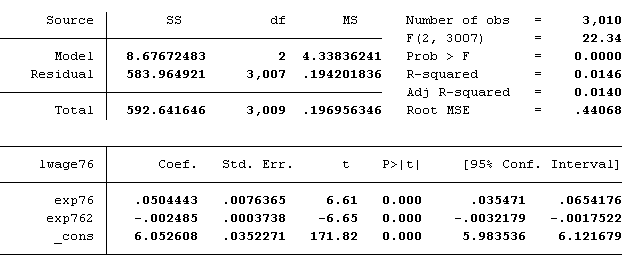
\includegraphics[width=0.7\linewidth]{screenshot002}
	%	\caption{}
	\label{fig:screenshot001}
\end{figure}

Second, we run locally weighted scatterplot smoothing (LOWESS) with bandwidth 0.8. 

Plotting both predicted values on a same plot, where red line represents polynomial fit estimated with OLS and  a green line represents the smoothed curve by non-parametric method, we can see, that the predictions differ insignificantly. That means that second-order polynomial is a reasonable model, as the shape of a curve is exactly the same as a non-parametric model would suggest. However, LOWESS fit shows, that a linear fit would not be a suitable model here. 



\begin{figure}[H]
	\centering
	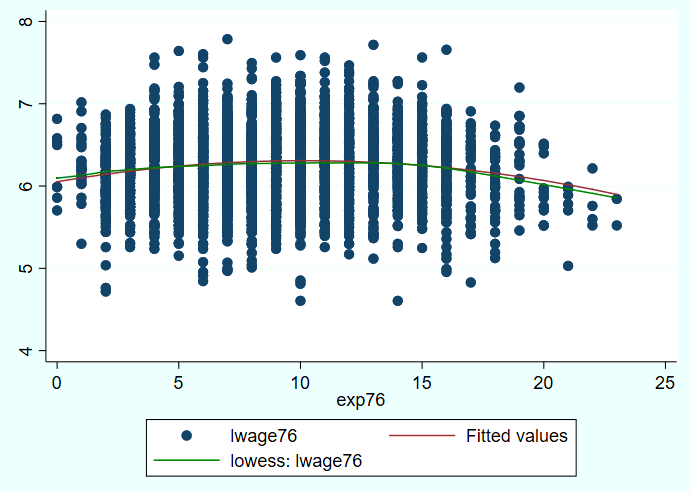
\includegraphics[width=0.7\linewidth]{screenshot004}
	%	\caption{}
	\label{fig:screenshot001}
\end{figure}


STATA code:

\begin{verbatim}
reg lwage76 exp76 exp762
predict preg
lowess lwage76 exp76, generate (pnonp)
twoway (scatter lwage76 exp76) (line preg exp76, sort) 
(line pnonp exp76, sort lcolor(green))
\end{verbatim}



\end{document}
